\outline{1}{Diminishing Returns of Dose and Duration of Rehabilitation Post-Stroke as Revealed by Dynamic Mixed Effect Model}
\chapter{Diminishing Returns of Dose and Duration of Rehabilitation Post-Stroke as Revealed by Dynamic Mixed Effect Model}
\label{cha:dose}


\outline{2}{Introduction}
\section{Introduction}
Observational rehabilitation studies are important as they shed light on effective factors in rehabilitation.
Among the multi-variate techniques used to analyze data from these studies are regression models, including mixed effect models that account for individual variations. 
Regression models have been used to predict stroke recovery \cite{19-22} and response to interventions {23,24,25}. 
Such models exhibit room for improvement because they are based on aggregate clinical scales, but also, we hypothesize, because they do not model the time-varying processes of recovery. 
In contrast, dynamical models naturally encode time in differential equations that model “changes in states”. 

State Space Model (SSM) is a dynamic model that describes a dynamic process via state vectors in state space \cite{}.
The field of motor adaptation and learning constantly uses SSM to model motor learning and adaptation data.
Unlike regression models, state-space models can describe processes that respond, simultaneously or with a latency, to time-varying inputs or stimuli.
This approach will allow us to test for causal relationships between training, learning, and recovery. 
In addition, the model will allow us to obtain a detailed time course of time window of plasticity. 
Although never applied to stroke recovery, such models have been applied successful to model the action of drugs on a range of diseases \cite{80,81}. 

One of the challenges of using SSM is to incorporate random effects into SSM, which is computationally not trivial and offered by few statistics toolboxes \cite{}.
Random effects in SSM is desirable especially in observational rehabilitation studies because of the high variability in stroke rehabilitation.
In this work, we circumvent this challenge by converting state space model to ordinary differential equation.
We show that under certain conditions, state space equation is equivalent to differential equation, and therefore share the same solution, which is a nonlinear function.
We then use nonlinear mixed effect model to estimate the parameters in this nonlinear solution.


\outline{2}{Methods}
\section{Methods}
\subsection{DOSE Trial}
In this study, we analyzed the data from Dose Optimization for Stroke Evaluation (DOSE) clinical trial \cite{}. 
40 post-stroke individuals participated in this study. 
Fig. \ref{fig:dosetimeline} shows the timeline of the study: participants receive two baseline tests before three periods of therapy intervention, followed by 6 follow-up tests. 
Each period of therapy intervention lasts 1 week, right after a pre-training test and followed by a post-training test. 
There is one month between intervention periods and follow-up tests. 
The whole study lasts 37 weeks for each participant.

\begin{figure}
	\centering
	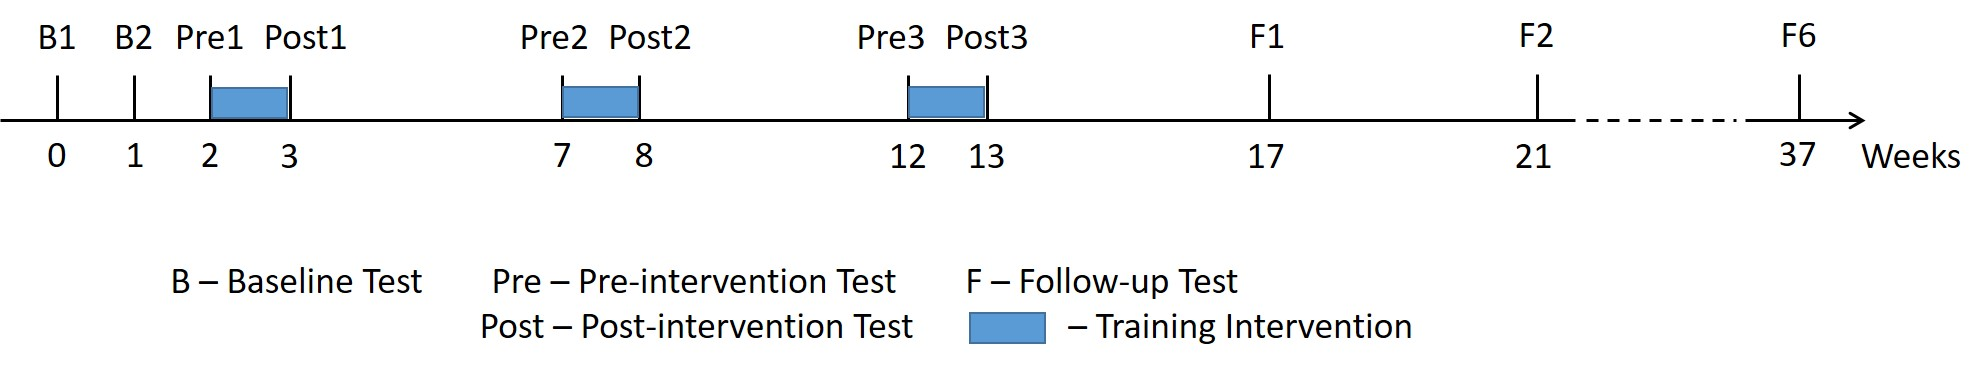
\includegraphics[width=1\linewidth]{figures/dosetimeline}
	\caption[DOSE Study Timeline]{The timeline of DOSE study. Each tick represents a test. Three training intervention periods in between three pairs of pre and post tests.}
	\label{fig:dosetimeline}
\end{figure}

Participants were grouped randomly into four groups with different dosage of therapy training during the intervention period: zero, low, moderate, and high therapy dose, measured by the amount of time of treatment: 0, 5, 10, 20 hours per week.

In each test, participants received Wolf Motor Function Test (WMFT) and Bilateral Arm Reaching Test (BART), as well as an interview of Motor Activity Log (MAL). 
Concerning the BART and WMFT tests last as long as 2 hours, we include this testing effect into the hours of training, so that we have 22, 12, 7, 2 hours of training for the four groups.

\subsection{State Space Model to Nonlinear Mixed Effect Model}
In the field of motor perturbation adaptation, state space model is adopted to model learning behavior [cite]. 
In particular, the state of the system $ x_k $ at trial $ k $ follows 
\begin{equation}\label{ssm}
	x_{k+1} = Ax_k + Bu_k
\end{equation}
Where $ A $ represents retention, and often takes a value slightly smaller than 1; 
where as B, slightly bigger than 0, represents learning due to input $ u_k $ {often indicating the error in motor perturbation adaptation).
This formula can be written as a differential equation:
\begin{equation}
	\frac{\Delta x_k}{\Delta t} = \frac{x_{k+1}-x_k}{\Delta t} = \frac{(A-1)x_k}{\Delta t} + \frac{Bu_k}{\Delta t}
\end{equation}
Omit index $ k $ and let $ a = (A-1)/\Delta t $, $ b = B/\Delta t $ and $ \Delta t\rightarrow 0 $, we have
\begin{equation}\label{oode}
	\frac{dx(t)}{dt} = ax(t)+bu(t)
\end{equation}
The solution to this differential equation is in general
\begin{equation}\label{generalsolution}
	x = x_0e^{at} + b\int_0^t e^{a(t-\tau)}u(\tau)d\tau
\end{equation}
If $ a $ is small comparing to the time scale concerned (that is to say $ |at_{\text{max}}| \ll 1 $) and $ b $ is comparibly small to $ a $ (that is to say $ \text{lim}\frac{bu_\text{max}}{ax_\text{max}} \leqslant \text{const.} $), then the first order approximation to this solution is
\begin{equation}\label{specialsolution}
	x = x_0 + x_0at + b \int_0^t u(\tau)d\tau
\end{equation}
Let $ c=x_0 a $, the original differential equation \ref{oode} becomes
\begin{equation}
	\frac{dx(t)}{dt} = bu(t) + c
\end{equation}
To isolate the effect of training input $ u(t) $, we further assume that c can be ignored when $ u(t) \neq 0 $, i.e.
\begin{equation}\label{fode}
	\frac{dx(t)}{dt} = bu(t) + cv(t)
\end{equation}
where
\begin{equation}
v(t) = 
\begin{cases}
	1, & \text{if}\ u(t) = 0 \\
	0, & \text{otherwise}
\end{cases}
\end{equation}
Or, in logical notation, $ v(t) = \sim u(t) $. 
This assumption would be further justified later when we show $ bu(t) $ is much larger than $ c $.

Denote the solution to Eqn. \ref{fode} as nonlinear function $ x=f(x_0,b,c,t) $, we estimate the mixed effect model as
\begin{equation}\label{eqn:nonlinear}
	x_i (t)=f(x_{0i},b_i,c_i,t) + \epsilon_i (t)
\end{equation}
where $ x_{0i} $, $ b_i $, $ c_i $ are the mixed effect parameters which can vary from individual to individual (cite Bates).
$ \epsilon_i (t) $ is the residual. 
We choose different mixed effects on $ b_i $ and $ c_i $ to investigate different aspects of training mentioned above.

\textbf{Training Efficacy and Efficiency.}
To estimate the efficacy of training (the overall effect of training), we let $ u(t)=1 $ during the intervention periods as shown in Fig. \ref{fig:dosefigure2}A. 
To estimate the efficiency of training (the effect of training per hour), we let $ u(t) $ to be the number of treatment hours corresponding to the group, as shown in Fig. \ref{fig:dosefigure2}B. 

\begin{figure}
	\centering
	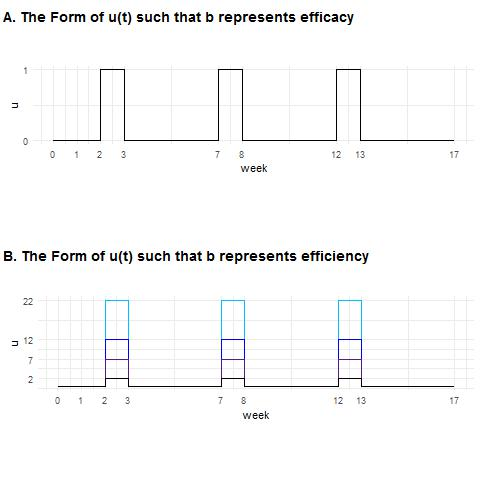
\includegraphics[width=0.7\linewidth]{figures/dosefigure2}
	\caption[Efficacy and Efficiency]{Different training input $u(t)$ for estimating Efficacy and Efficiency. In Panel A, $u(t)$ is either 1 or 0. In Panel B, $u(t)$ is the number of hours received in that training period. $u(t)$ is different for different groups.}
	\label{fig:dosefigure2}
\end{figure}

To investigate how training efficacy and efficiency depends on dosage of training, we use a linear formula for the mixed effects of $ b_i $ and $ c_i $:
\begin{eqnarray}\label{eqn:mixedeffect}
	b_i &=& \beta_1^b + \beta_2^b D_i + \delta_i^b   \nonumber \\
	c_i &=& \beta_1^c + \beta_2^c D_i + \delta_i^c   \\
	x_{0i} &=& \beta_1^{x_0} + \beta_2^{x_0} A_i + \delta_i^{x_0} \nonumber
\end{eqnarray}
where $ D_i $ is the dosage of training (number of hours per week) participant $ i $ received, 
$ A_i $ is certain clinical assessment before the training, e.g the initial FM score and/or CST of participant $ i $, 
$ \beta $ are fixed effects and $ \delta_i $ are random effects. 
Indexes on the shoulder indicates the parameter to which this fixed or random effect belongs.

In the case when we take the dosage of training as categorical variable, i.e. how efficacy and efficiency depends on the four groups, the formula becomes
\begin{equation}
	b_i = \beta_1^b + \beta_2^b D_{i2} + \beta_3^b D_{i3} + \beta_4^b D_{i4} + \delta_i^b
\end{equation}
Where $ D_{ij} $ is 1 when participant i belongs to group j, 0 otherwise. The formula for $ c_i $ is in the same structure.

\textbf{The Timing of Training}
To look at the effect of training at different period, we further assume $ b $ and $ c $ can take different values at different intervention periods. 
We applied this assumption in two ways: 1) A linear dependence of $ b $ (and $ c $) on training period $ k (k=1,2,3) $, namely
\begin{eqnarray}\label{eqn:timingcat}
	b(k) &=& b_0 + b_t (k-1) \nonumber  \\
	c(k) &=& c_0 + c_t (k-1)
\end{eqnarray}
So that we have two more parameters than Eqn. \ref{fode}. 

Due to insufficient data points (too few data points at each training period), we simplify the mixed effects of $ b(k) $ and $ c(k) $:
\begin{eqnarray}
	b_0 &=& \beta_1^b + \delta_i^b \\
	b_t &=& \beta_2^b
\end{eqnarray}
The formula for $ c_0 $ and $ c_t $ is in the same structure.

2) Independent values of $ b $ and $ c $ at different training period, namely
\begin{equation}
	b = b_k, c = c_k, k = 1,2,3
\end{equation}
So that we have four more parameters than Eqn. \ref{fode}. 

We use maximum likelihood to estimate parameters.


\section{Results}
We first apply the mixed effect model to MAL data. 
The mixed effect models fit the data quite well; 
as an example, in Fig. \ref{fig:dosefitA} and Fig. \ref{fig:dosefitB} we show the model fitting of efficiency (Fig. \ref{fig:dosefigure2}B), with full mixed effects in Eqn. \ref{eqn:mixedeffect}:

\begin{figure}
	\centering
	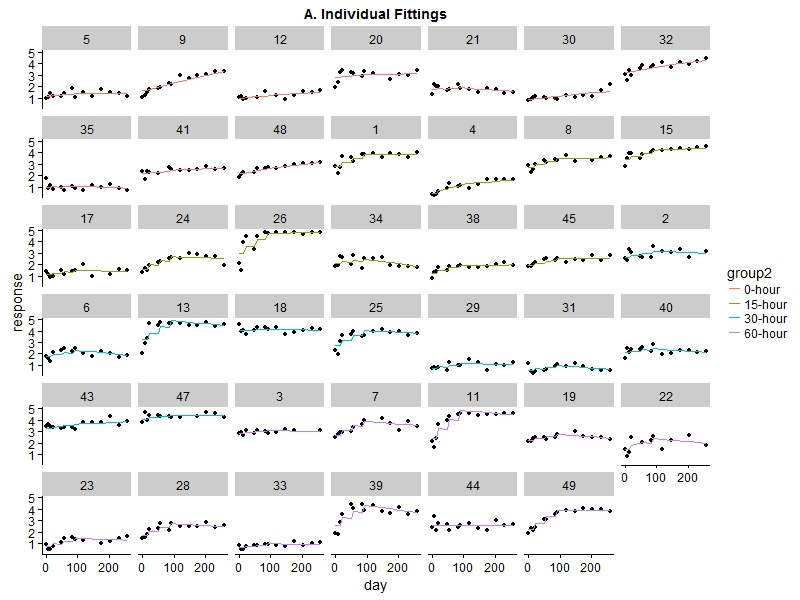
\includegraphics[width=1\linewidth]{figures/dosefitA}
	\caption[Individual Fitting]{Individual Fitting of MAL}
	\label{fig:dosefitA}
\end{figure}
\begin{figure}
	\centering
	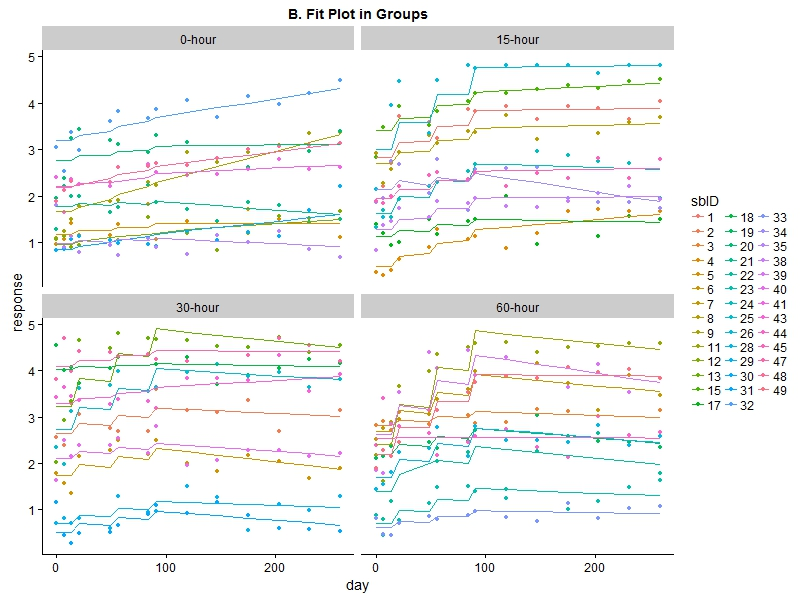
\includegraphics[width=1\linewidth]{figures/dosefitB}
	\caption[Plot by Groups]{MAL individual fitting plotted in four groups}
	\label{fig:dosefitB}
\end{figure}

\subsection{Training Efficacy and Efficiency}
The fitting result of full mixed effects (Eqn. \ref{eqn:mixedeffect}) for efficacy and efficiency is shown in table \ref{tab:ee}.


% Table created by stargazer v.5.2 by Marek Hlavac, Harvard University. E-mail: hlavac at fas.harvard.edu
% Date and time: Mon, May 01, 2017 - 4:49:27 PM
% Requires LaTeX packages: dcolumn 
\begin{table}[!htbp] \centering 
	\caption{Efficacy vs Efficiency} 
	\label{tab:ee} 
	\begin{tabular}{@{\extracolsep{5pt}}lD{.}{.}{-3} D{.}{.}{-3} } 
		\\[-1.8ex]\hline 
		\hline \\[-1.8ex] 
		& \multicolumn{2}{c}{\textit{Dependent variable:}} \\ 
		\cline{2-3} 
		\\[-1.8ex] & \multicolumn{2}{c}{MAL} \\ 
		\\[-1.8ex] & \multicolumn{1}{c}{(1)} & \multicolumn{1}{c}{(2)}\\ 
		\hline \\[-1.8ex] 
		$ x_0$.(Intercept)  & -0.815$ $(0.531) & -0.849$ $(0.537) \\ 
		$ x_0$.FM  & 0.067^{***}$ $(0.012) & 0.068^{***}$ $(0.012) \\ 
		b.(Intercept) & 0.018$ $(0.009) & 0.006^{***}$ $(0.001) \\ 
		b.dose & 0.002^{*}$ $(0.001) & -0.0002^{*}$ $(0.0001) \\ 
		c.(Intercept) & 0.001$ $(0.001) & 0.001$ $(0.001) \\ 
		c.dose & -0.0001^{*}$ $(0.0001) & -0.0001^{*}$ $(0.0001) \\ 
		\hline \\[-1.8ex] 
		Observations & \multicolumn{1}{c}{557} & \multicolumn{1}{c}{557} \\ 
		Log Likelihood & \multicolumn{1}{c}{-282.856} & \multicolumn{1}{c}{-289.240} \\ 
		Akaike Inf. Crit. & \multicolumn{1}{c}{591.711} & \multicolumn{1}{c}{604.479} \\ 
		Bayesian Inf. Crit. & \multicolumn{1}{c}{647.904} & \multicolumn{1}{c}{660.673} \\ 
		\hline 
		\hline \\[-1.8ex] 
		\textit{Note:}  & \multicolumn{2}{r}{$^{*}$p$<$0.05; $^{**}$p$<$0.01; $^{***}$p$<$0.001} \\ 
	\end{tabular} 
\end{table} 

$ \beta_1^b $ (b.dose in the table) is positive for efficacy, but negative for efficiency, which indicates that training efficacy increases with dose, while efficiency decreases.

\subsection{Timing of training}
The fitting result with timing effect \ref{eqn:timingcat}, but without dose fixed effect, is shown in table \ref{tab:timing}.
Both $ b_t $ and $ c_t $ are significantly negative, indicating the effect of training decreases as training progresses.

% Table created by stargazer v.5.2 by Marek Hlavac, Harvard University. E-mail: hlavac at fas.harvard.edu
% Date and time: Mon, May 01, 2017 - 5:00:11 PM
% Requires LaTeX packages: dcolumn 
\begin{table}[!htbp] \centering 
	\caption{Timing Effect} 
	\label{tab:timing} 
	\begin{tabular}{@{\extracolsep{5pt}}lD{.}{.}{-3} } 
		\\[-1.8ex]\hline 
		\hline \\[-1.8ex] 
		& \multicolumn{1}{c}{\textit{Dependent variable:}} \\ 
		\cline{2-2} 
		\\[-1.8ex] & \multicolumn{1}{c}{MAL} \\ 
		\hline \\[-1.8ex] 
		$ x_0 $.(Intercept) & -0.855$ $(0.533) \\ 
		$ x_0 $.FM & 0.067^{***}$ $(0.012) \\ 
		$ b_0 $ & 0.004^{***}$ $(0.001) \\ 
		$ b_t $ & -0.002^{***}$ $(0.0003) \\ 
		$ c_0 $ & 0.004^{*}$ $(0.002) \\ 
		$ c_t $ & -0.002^{*}$ $(0.001) \\ 
		\hline \\[-1.8ex] 
		Observations & \multicolumn{1}{c}{557} \\ 
		Log Likelihood & \multicolumn{1}{c}{-276.891} \\ 
		Akaike Inf. Crit. & \multicolumn{1}{c}{579.782} \\ 
		Bayesian Inf. Crit. & \multicolumn{1}{c}{635.976} \\ 
		\hline 
		\hline \\[-1.8ex] 
		\textit{Note:}  & \multicolumn{1}{r}{$^{*}$p$<$0.05; $^{**}$p$<$0.01; $^{***}$p$<$0.001} \\ 
	\end{tabular} 
\end{table} 